\section{Event-Level Correction}
\label{sec:correction}

When the video is right but some events are wrong, the user should not need to rewrite the query.
We measure how quickly a user can repair the path by acting on one event at a time, with every action turned into a constraint on the same cached score matrix.

\begin{figure}[t]
\centering
\resizebox{\textwidth}{!}{% Editable vector layout; photographs are original, unchanged corpus JPEGs.
\begin{tikzpicture}[x=1mm,y=1mm,
  font=\sffamily\fontsize{8}{9}\selectfont,
  ink/.style={text=corrInk},
  flow/.style={-{Stealth[length=1.7mm]},draw=corrSlate,line width=.7pt},
  heading/.style={anchor=west,font=\sffamily\bfseries\fontsize{9}{10}\selectfont,text=corrInk},
  small/.style={font=\sffamily\fontsize{7}{8}\selectfont,text=corrSlate},
  button/.style={rounded corners=1.3mm,line width=.6pt,minimum width=34mm,minimum height=6mm,inner sep=0pt}
]
\definecolor{corrInk}{HTML}{172B48}
\definecolor{corrSlate}{HTML}{61758A}
\definecolor{corrBlue}{HTML}{4088BC}
\definecolor{corrLine}{HTML}{BDD3E6}
\definecolor{corrLav}{HTML}{A59ACC}
\definecolor{corrAccent}{HTML}{CE6541}
\definecolor{corrGreen}{HTML}{608B77}
\path[use as bounding box] (0,0) rectangle (122,76);

% Inspection occupies one band; all four frames come from the same video.
\filldraw[fill=blue!2,draw=corrLine,rounded corners=2mm,line width=.7pt]
  (0,34) rectangle (122,76);
\node[heading] at (4,72) {1\quad Inspect one event};
\node[small,anchor=east] at (118,72) {$E_2$: add lime zest and juice};
\draw[corrLine,line width=.4pt] (4,68.5) -- (118,68.5);
\node[ink,anchor=west] at (4,65) {Current frame};
\node[ink,anchor=west] at (34,65) {Alternatives};
\foreach \xx/\stamp in {4/172,34/176,64/182,94/188}{
  \fill[corrInk,rounded corners=.65mm] (\xx,47.4) rectangle ++(24,15.2);
  \foreach \p in {0,...,10}{
    \fill[white!80!corrLine] (\xx+.8+2.1*\p,47.75) rectangle ++(1.1,.55);
    \fill[white!80!corrLine] (\xx+.8+2.1*\p,61.7) rectangle ++(1.1,.55);
  }
  \node[inner sep=0pt,anchor=south west] at (\xx+.5,48.35)
    {\includegraphics[width=23mm]{figures/correction-keyframes/L26_V422_\stamp s.jpg}};
  \node[small] at (\xx+12,45) {\stamp\,s};
}
\draw[corrAccent,rounded corners=.9mm,line width=1pt] (63.5,46.9) rectangle (88.5,63.1);

% The controls are mutually exclusive; Use is active in this example.
\node[button,draw=corrGreen!60,fill=white,text=corrGreen] (keep) at (21,39) {\hspace{3mm}Keep};
\draw[corrGreen,line width=.8pt,line cap=round,line join=round]
  (11,39) -- (12.2,37.8) -- (14.3,40.2);
\node[button,draw=corrAccent,fill=corrAccent!9,text=corrAccent,font=\sffamily\bfseries\fontsize{8}{9}\selectfont]
  (use) at (61,39) {\hspace{3mm}Use 182\,s};
\draw[corrAccent,line width=.75pt,line join=round]
  (48.8,40.6) -- (48.8,37) -- (49.9,38) -- (50.8,36.8) -- (51.6,37.3) -- (50.7,38.5) -- (52,38.6) -- cycle;
\node[button,draw=corrSlate!45,fill=white,text=corrSlate] (reject) at (101,39) {\hspace{3mm}Reject};
\draw[corrSlate,line width=.7pt,line cap=round] (89.8,37.8) -- (92.2,40.2) (89.8,40.2) -- (92.2,37.8);

\draw[flow,draw=corrAccent,dashed,rounded corners=1mm]
  (use.south) -- (61,31.5) -- (25,31.5) -- (25,29);
\filldraw[fill=corrLav!4,draw=corrLav!55,rounded corners=2mm,line width=.7pt]
  (0,0) rectangle (122,29);
\node[heading] at (4,25) {2\quad Constrain cached $S_v$};
\node[heading] at (74,25) {Updated event trail};
\node[small] at (25,20.6) {Video timeline $\rightarrow$};

% Schematic scores: fixing E2 leaves just the selected column admissible.
\foreach \row in {0,1,2}{
  \foreach \col in {0,...,9}{
    \pgfmathtruncatemacro{\shade}{mod(13*\col+23*\row+7*\row*\col,45)+12}
    \fill[corrLav!\shade!white] (8+3.4*\col,8+3.5*\row) rectangle ++(3.4,3.5);
  }
}
\foreach \col in {0,1,2,3,4,6,7,8,9}{
  \fill[white,opacity=.9] (8+3.4*\col,11.5) rectangle ++(3.4,3.5);
}
\foreach \col in {0,...,10}{\draw[corrLine,line width=.25pt] (8+3.4*\col,8) -- ++(0,10.5);}
\foreach \row in {0,...,3}{\draw[corrLine,line width=.25pt] (8,8+3.5*\row) -- ++(34,0);}
\node[small,anchor=east] at (7,16.75) {$E_1$};
\node[small,anchor=east,text=corrAccent] at (7,13.25) {$E_2$};
\node[small,anchor=east] at (7,9.75) {$E_3$};
\draw[corrSlate!70,densely dashed,line width=.7pt] (13.1,16.75) -- (16.5,13.25) -- (36.9,9.75);
\draw[corrBlue,line width=1pt] (16.5,16.75) -- (26.7,13.25) -- (33.5,9.75);
\foreach \xx/\yy in {16.5/16.75,33.5/9.75}{\fill[corrBlue] (\xx,\yy) circle (.65mm);}
\draw[corrAccent,line width=.85pt] (25,11.5) rectangle ++(3.4,3.5);
\fill[corrAccent] (26.7,13.25) circle (.7mm);
\node[small,text=corrAccent] at (26.7,5.5) {182\,s};
\draw[corrSlate!70,densely dashed,line width=.7pt] (4,2.5) -- (8,2.5);
\node[small,anchor=west] at (9,2.5) {Old};
\draw[corrBlue,line width=.9pt] (22,2.5) -- (26,2.5);
\node[small,anchor=west] at (27,2.5) {New};

\draw[flow] (43,13.5) -- (47,13.5);
\filldraw[draw=corrLine,fill=white,rounded corners=1.5mm,line width=.65pt] (48,7.5) rectangle (67,20);
\draw[corrBlue,line width=.8pt,line join=round] (52,16) -- (55,17) -- (59,18) -- (63,19);
\foreach \xx/\yy in {52/16,55/17,59/18,63/19}{\fill[corrBlue] (\xx,\yy) circle (.5mm);}
\node[ink,font=\sffamily\bfseries\fontsize{8}{9}\selectfont] at (57.5,11.2) {Re-run DP};
\node[small] at (57.5,3.8) {No index access};
\draw[flow] (68,13.5) -- (72,13.5);

% Real photographs in a schematic sequence; orange identifies the fixed event.
\foreach \xx/\stamp/\ev in {74/172/1,90/182/2,106/186/3}{
  \node[small] at (\xx+7,21.8) {$E_{\ev}$};
  \fill[corrInk,rounded corners=.5mm] (\xx,10.8) rectangle ++(14,9.1);
  \node[inner sep=0pt,anchor=south west] at (\xx+.3,11.4)
    {\includegraphics[width=13.4mm]{figures/correction-keyframes/L26_V422_\stamp s.jpg}};
  \node[small] at (\xx+7,8.2) {\stamp\,s};
}
\draw[corrAccent,rounded corners=.6mm,line width=.85pt] (89.6,10.4) rectangle (104.4,20.3);
\node[small,text=corrAccent] at (97,3.8) {$E_2$ fixed; others may move};
\end{tikzpicture}
}
\caption{Event-level correction with real corpus keyframes and schematic scores and paths. \emph{Keep} fixes the current frame; \emph{Use} fixes an alternative; \emph{Reject} removes the current timestamp cell bounded by neighboring midpoints. Here \emph{Use} fixes $E_2$ at 182\,s, and DP re-decodes all events on cached $S_v$ without index access (grey: old path; blue: new path). Three of the $k$ alternatives are shown. SHI~\cite{nguyen2027shi} implements these actions.}
\label{fig:trail}
\end{figure}


\paragraph{Actions and decoding.}
For a selected event $E_i$ (Fig.~\ref{fig:trail}) the user sees its current frame and $k$ alternatives and takes one of three actions.
\emph{Keep} fixes $E_i$ to its current frame.
\emph{Use} fixes $E_i$ to one of the alternatives.
\emph{Reject} removes from $E_i$'s admissible frames the cell around the current frame bounded by the midpoints to its neighboring timestamps, the same rejection unit as the EventTrail interface of SHI~\cite{nguyen2027shi}.
Fixed events and rejected cells form a mask on $S_v$, and the DP of Sect.~\ref{sec:benchmark} is re-run under the mask.
Re-decoding never touches the corpus index, so the decoder latency per action is about one millisecond, against a median of 3.8\,s for a new search; this is computation time only and excludes the time a user needs to inspect frames and decide.

\paragraph{Simulated user.}
An oracle user who knows the annotated intervals repeatedly selects an event that is not yet fixed: if its frame is correct it keeps it; otherwise it uses a correct alternative if one is shown and rejects the current frame if not.
We vary three factors.
\emph{Proposals}: the $k$ alternatives are either the highest-scoring frames of $E_i$ at least 5\,s apart (\emph{local}), or the focus frames of the $k$ best complete paths through distinct frames of $E_i$, computed by forward--backward max-marginals (\emph{path}).
\emph{Order}: events are inspected left to right, in random order (10 seeds), or in increasing order of a per-event confidence, the score lost by forcing the event to its best distinct alternative.
\emph{Propagation}: after an action the whole path is re-decoded (\emph{joint}), or only the touched event is re-decoded while the others stay where they are (\emph{frozen}).
We report the fraction of queries whose path is entirely correct after at most $B$ actions, H@$B$, and the number of frames presented (the current frame plus $k$ alternatives per action).
The simulation stops as soon as the whole path is correct, including events the user has not yet confirmed, so a query that is correct initially costs no presentations; presentation counts are therefore effort under oracle stopping, not measured human effort.
As a baseline without the decoder (\emph{no DP}), each event starts at its highest-scoring frame and actions change only the touched event, without order constraints.
Frozen re-decoding keeps the DP starting path and re-places the touched event between its fixed neighbors, but does not propagate to untouched events; if the user's choice falls outside the neighbors, it is applied anyway, as a local editor would (3 of 40 queries for each $k$, one of which ends solved with an out-of-order path).

\begin{table}[t]
\centering
\caption{Whole-sequence correctness (\%) after at most $B$ actions on 40 queries with the correct video given and an oracle user, $k$ alternatives per action. The lower block uses joint re-decoding; random order averages 10 seeds over the same 40 queries. H@0 is 25.0 with DP and 10.0 without.}
\label{tab:correction}
\begin{tabular}{llcccccccc}
\toprule
 & & \multicolumn{4}{c}{$k=4$} & \multicolumn{4}{c}{$k=8$} \\
\cmidrule(lr){3-6}\cmidrule(lr){7-10}
Proposals & Order & H@1 & H@2 & H@3 & H@5 & H@1 & H@2 & H@3 & H@5 \\
\midrule
\multicolumn{2}{l}{no DP, local, sequential} & 15.0 & 25.0 & 37.5 & 37.5 & 17.5 & 32.5 & 42.5 & 47.5 \\
\multicolumn{2}{l}{frozen, local, sequential} & 25.0 & 47.5 & 55.0 & 60.0 & 27.5 & 50.0 & 57.5 & 67.5 \\
\midrule
local & sequential & 25.0 & 47.5 & 57.5 & 62.5 & 27.5 & 50.0 & 60.0 & 70.0 \\
local & random     & 32.7 & 49.8 & 57.8 & 66.8 & 34.5 & 55.2 & 66.2 & 75.2 \\
local & confidence     & 27.5 & 50.0 & 60.0 & 62.5 & 27.5 & 57.5 & 65.0 & 70.0 \\
path  & sequential & 27.5 & 50.0 & 60.0 & 65.0 & 30.0 & 52.5 & 62.5 & 67.5 \\
path  & random     & 33.5 & 48.5 & 61.5 & 66.2 & 35.2 & 53.8 & 68.2 & 75.2 \\
path  & confidence     & 27.5 & 50.0 & 60.0 & 67.5 & 30.0 & 52.5 & 65.0 & 70.0 \\
\bottomrule
\end{tabular}
\end{table}


\begin{figure}[t]
\centering
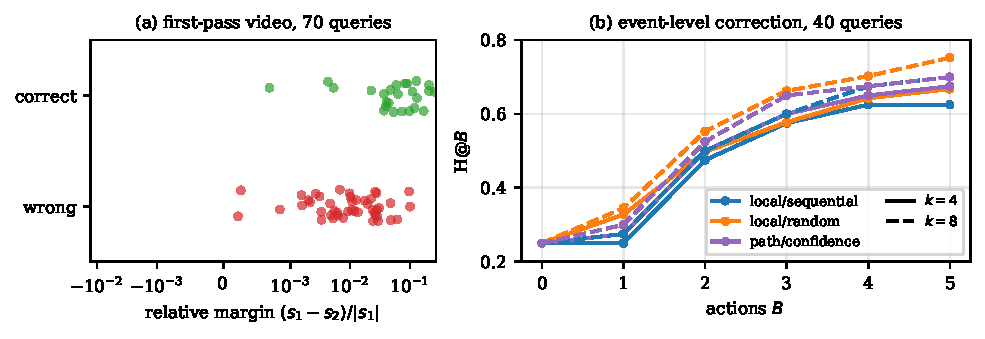
\includegraphics[width=\linewidth]{figures/results.pdf}
\caption{(a) Relative margin between the best path and the best path of a different video, for first passes that retrieved the correct or a wrong video (70 queries, symmetric log scale). (b) Whole-sequence correctness after at most $B$ actions for three proposal/order settings, $k=4$ (solid) and $k=8$ (dashed).}
\label{fig:results}
\end{figure}

\paragraph{Correction headroom under oracle feedback.}
Table~\ref{tab:correction} and Fig.~\ref{fig:results}b show that, with the correct video given, five actions raise whole-sequence correctness from 25\% to 62.5--67.5\% with four alternatives and to 67.5--75.2\% with eight; the upper end is random order, whose 10 seeds are rollouts over the same 40 queries.
The gain holds in every subset (path proposals, sequential order, $k=4$): from 23\% to 62\% on the first set, whose submissions name a single video, 14\% to 86\% on the second, 40\% to 67\% on the third, and 0\% to 40\% on the five TRAKE queries.
The number of alternatives shown per action matters more than how they are chosen, but it is not free: with sequential order 14.1 frames per query are presented on average with $k=4$ and 24.3 with $k=8$.

\paragraph{Where the decoder helps.}
With the same proposal rule and action budget but no DP, H@5 is 37.5\% ($k=4$) and 47.5\% ($k=8$), against 62.5\% and 70.0\% with joint re-decoding, and more frames are presented (18.8 and 31.5).
The difference is paired and one-sided: DP solves 10 queries ($k=4$) and 9 ($k=8$) that the baseline does not, and the baseline solves none that DP misses (95\% bootstrap interval of the difference 12.5--40 points for $k=4$).
Frozen re-decoding already reaches 60\% and 67.5\%, so most of the gap comes from the DP starting path (25\% against 10\% before any action) and from placing a re-decoded event between its neighbors (counting the out-of-order frozen path as a failure lowers frozen by 2.5 points); propagating a correction to untouched events adds one query for each $k$ (95\% interval 0--7.5 points).
Because the proposals depend on the current frame, which differs between the settings, the user is not shown identical alternatives in all three.

\paragraph{Where five actions suffice.}
With two to four events per query, H@5 ($k=4$, local, sequential) is 80\% for two-event queries, 53\% for three, and 50\% for four.
By the number of wrongly placed events in the initial path, it is 80\% with one and 78\% with two, but 0\% with three or four: the budget repairs paths with a few errors, not paths that are mostly wrong.

\paragraph{End to end.}
The numbers above assume the correct video.
If the user corrects only the top-ranked video and a wrong video counts as a failure, whole-sequence correctness over the 40 queries rises from 10\% to 35\% for both $k=4$ and $k=8$, because the correct video is ranked first for only 16 queries; this is a computation over the stored runs, not a separate full-pipeline experiment.
This is why the two mechanisms are complementary: correction pays off only after the video is right.

\paragraph{What did not help.}
Three refinements that we expected to reduce effort showed no consistent improvement; on 40 queries one query is 2.5 points, so the differences below are within a few queries.
\emph{Path proposals} were not consistently better than local ones: at H@5 they differ by $-2.5$ to $+5$ points across orders and $k$.
\emph{Confidence-ordered inspection} was not better than left-to-right or random order; the per-event confidence is only weakly related to errors (AUROC 0.61, Sect.~\ref{sec:failure_prediction}), so the user often inspects correct events first.
\emph{Propagation} barely mattered: frozen re-decoding reaches H@5 within 6 points of joint re-decoding in every setting.
Joint re-decoding does repair untouched events, 0.05--0.23 per query, but it breaks a similar number, 0.09--0.20 per query, so the effects cancel.
The evidence for the other events is too weak for a confirmed event to move them reliably, consistent with the frame-scoring bottleneck of Sect.~\ref{sec:diagnosis}.
